\documentclass[10pt]{beamer}
\usetheme[progressbar=frametitle]{metropolis}
\usepackage{amsmath}
\usepackage{amsfonts}
\usepackage{commath}
\usepackage{mathtools}
\usepackage{tabu}
\usepackage{booktabs}
\usepackage{bm}
\usepackage{xfrac}
\usepackage{subcaption}
\usepackage{graphicx}
\usepackage{pgfplots}
\usepackage{hyperref}
\hypersetup{pdfpagemode=FullScreen}

\newcommand{\RR}{\mathbb{R}}
\DeclarePairedDelimiter\ip{\langle }{\rangle}

\title{Diff Geo}
\subtitle{Gyroscopic Data Analysis Using SO(3)}
\date{\today}
\author{Nick Draper \and Jonathan Hayase}
\institute{Math 143 -- Differential Geometry Seminar -- Spring 2018}

\begin{document}

\maketitle

\begin{frame}{Table of contents}
    \setbeamertemplate{section in toc}[sections numbered]
    \tableofcontents[hideallsubsections]
\end{frame}

\section{Introduction}

\begin{frame} {Motivation}
Typical devices will usually contain a multitude of sensors for measuring properties that can be useful for modeling and analysis such as accelerations, rotational velocities, and magnetic fields ect. 
\begin{figure}
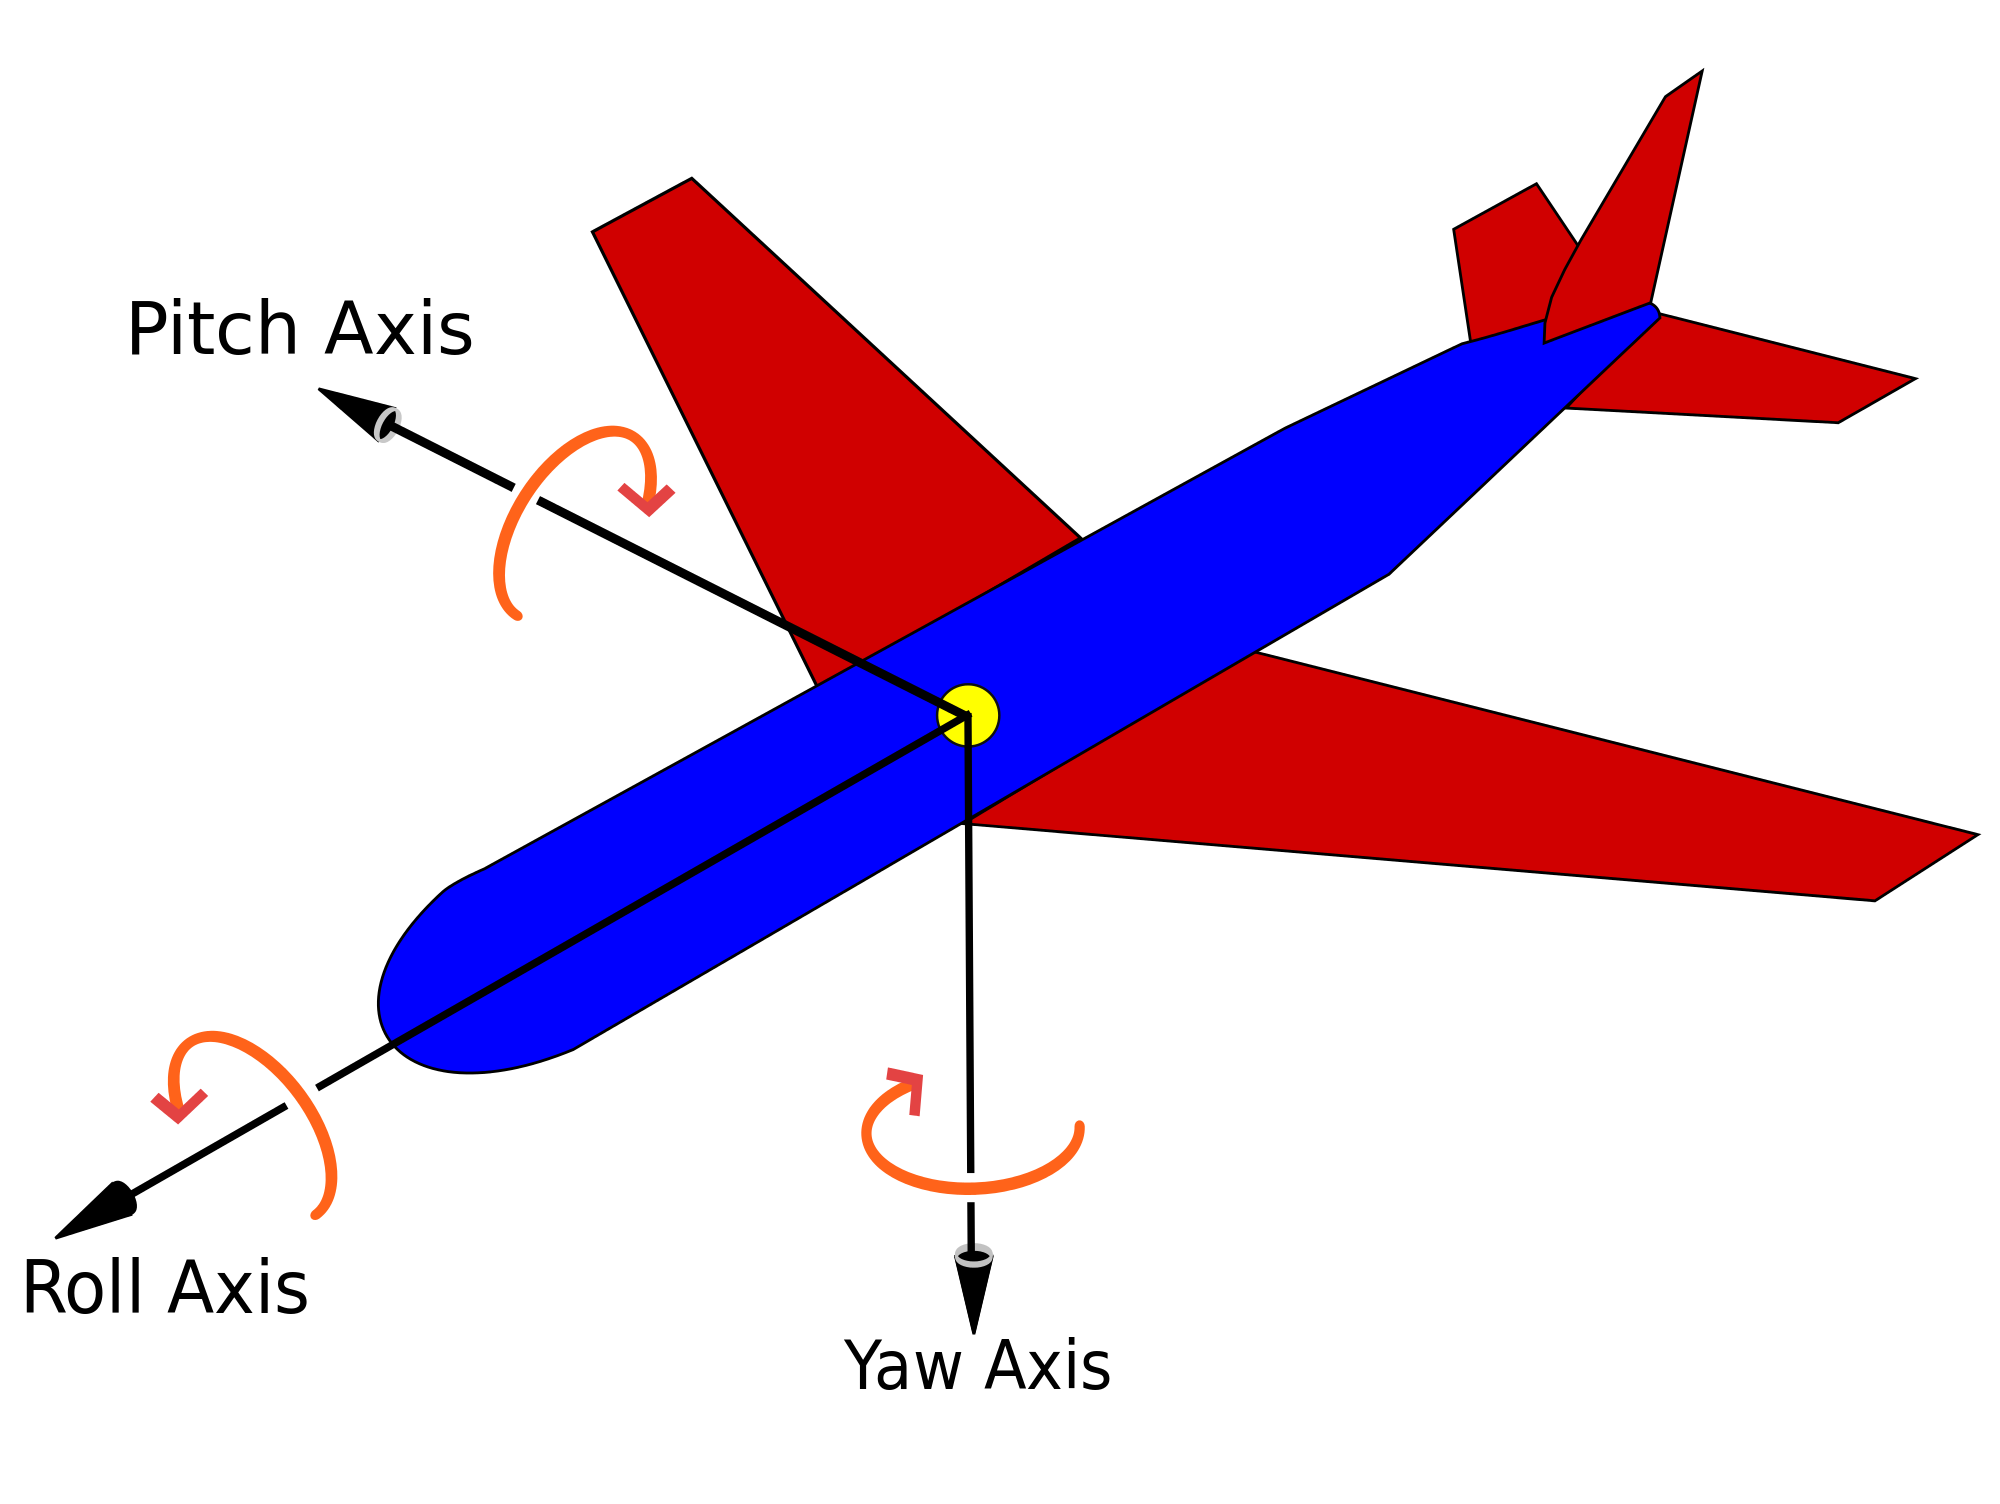
\includegraphics[scale=0.08]{images/plane.png}
\caption{Illustration of a plane with its corresponding axes of rotation labeled \cite{plane1}.}
\end{figure}
\end{frame}

\begin{frame} {Application}
We can capture such data from Android  cellphones and try to mathematically find patterns of what people are doing with their phone. 
\begin{figure}
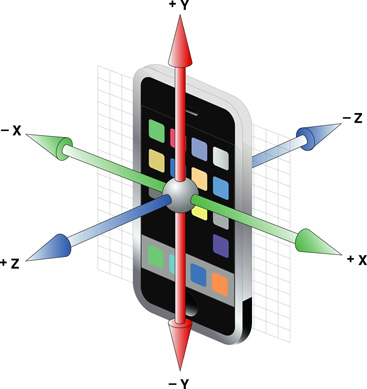
\includegraphics[scale=.4]{images/phone1.jpg}
\end{figure}
\end{frame}

\section{Dataset}

\begin{frame} {HMOG}
We will be using the hand movement, orientation, and
grasp (HMOG) dataset \cite{phone}. This dataset contains a set of behavioral features that allows for continuous authentication of Android smartphone users. 
\end{frame}

\begin{frame} {Users and Sessions}
The HMOG dataset contains data for over 100 users with each user having 24 sessions of data. The different sessions of data refer to different tasks described by the following.
\begin{enumerate}
\item Reading \& Sitting: \{1,7,13,19\}
\item Reading \& Walking: \{2,8,14,20\}
\item Writing \& Sitting: \{3,9,15,21\}
\item Writing \& Walking: \{4,10,16,22\}
\item Mapping \& Sitting: \{5,11,17,23\}
\item Mapping \& Walking: \{6,12,18,24\}
\end{enumerate}
\end{frame}

\begin{frame} {CSV Data Files}
From there the data is furthered separated into each of its sensor measurements. The following list is the available data files we have for each session. 
\begin{enumerate}
\item Accelerometer.csv
\item Gyroscope.csv
\item Magnetometer.csv
\item TouchEvent.csv
\item KeyPressEvent.csv
\item OneFingerTouchEvent.csv
\item PinchEvent.csv
\item ScrollEvent.csv
\item StrokeEvent.csv
\end{enumerate}
\end{frame}

\begin{frame} {Accelerometer Data}
The accelerometer file contains the following information.
\begin{itemize}
\item Absolute Time Stamps
\item Acceleration on the x-axis
\item Acceleration on the y-axis
\item Acceleration on the z-axis
\item Phone Orientation: \{0,1,3\}
\end{itemize}
\end{frame}

\begin{frame} {Gyroscope Data}
The gyroscope file contains the following information.
\begin{itemize}
\item Absolute Time Stamps
\item Angular speed about x-axis
\item Angular speed about y-axis
\item Angular speed about z-axis
\item Phone Orientation: \{0,1,3\}
\end{itemize}
\end{frame}

\begin{frame} {Magnetometer Data}
The magnetometer file contains the following information.
\begin{itemize}
\item Absolute Time Stamps
\item Ambient magnetic field in the x-axis
\item Ambient magnetic field in the y-axis
\item Ambient magnetic field in the z-axis
\item Phone Orientation: \{0,1,3\}
\end{itemize}
\end{frame}

\begin{frame} {Touch Event Data}
The touch event file contains the following information.
\begin{itemize}
\item Absolute Time Stamps
\item Pointer count: \{Single touch, Multi touch\}
\item Pointer ID: \{First pointer, Second pointer in multi touch\}
\item X location of touch
\item Y location of touch
\item Pressure of the touch 
\item Contact size of touch
\item Phone Orientation: \{0,1,3\}
\end{itemize}
\end{frame}

\begin{frame} {Key Press Event Data}
The key press event file contains the following information.
\begin{itemize}
\item Absolute Time Stamps
\item Press Type: \{Finger down, Finger up\}
\item Phone Orientation: \{0,1,3\}
\end{itemize}
\end{frame}

% \begin{frame} {One Finger Touch Event Data}
% The one finger touch event file contains the following information.
% \begin{itemize}
% \item Absolute Time Stamps
% \item Press Time
% \item Tap Type: \{First finger down of single tap, First finger down of double tap, Second finger down of double tap\}
% \item X location of touch
% \item Y location of touch
% \item Pressure
% \item Contact Size
% \item Phone Orientation: \{0,1,3\}
% \end{itemize}
% \end{frame}

\section{Error Sources}

\begin{frame}
Assuming we have perfect uniform time sampled data, there are still a number of errors that can appear in the data.
\begin{enumerate}
\item Bias
\item White Noise
\item Temperature Effects
\item Calibration
\item Bias Instability
\end{enumerate}
\end{frame}

\begin{frame}
\frametitle{Bias Error}
Bias is some marginal error $\epsilon$ that is incorporated when we try to integrate the data. The error is proportional to the time interval we integrate over.
\begin{equation*}
\theta(t) = \epsilon \cdot t
\end{equation*}
\end{frame}

\begin{frame}
\frametitle{White Noise Error}
White noise is a type of noise that has an associated standard deviation of $\sigma$. As we integrate this error is grows proportionally with the square root of time. 
\begin{equation*}
\sigma_{\theta}(t) = \sigma \cdot \sqrt{\partial t \cdot t}
\end{equation*}
\end{frame}

\begin{frame}
\frametitle{Temperature Effect Error}
Residual bias that depends on temperature. This residual bias is factored into the orientation which causes an error in the orientation data. This error is proportional with time.
\end{frame}

\begin{frame}
\frametitle{Calibration Error}
Calibration errors can be attributed to errors in the scale factors, alignments, and the gyro linearities. When integrating this kind of error, it is proportional to the rate and duration of motion.
\end{frame}

\begin{frame}
\frametitle{Bias Instability Error}
This kind of error can be attributed to bias fluctuations and can be modeled as a bias random walk. When integrating this kind of error, it results in a second-order random walk.  
\end{frame}

\begin{frame} {Sampling Issue}
Another challenge we must address for this project is the non-ideal timing issues with the data. The data is not uniformly sampled. 
\end{frame}

\begin{frame} {Sampling Issue}
\begin{figure}
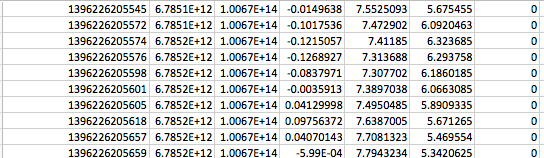
\includegraphics[scale=0.55]{images/data1.png}
\end{figure}
\end{frame}

\section{Orientation Theory}

\begin{frame}{Orientation Theory: Introduction}
  \begin{itemize}
  \item We have many sensors that yield data relevant to the phone's orientation.
  \item The most precise is the phone's gyroscope.
  \item We can find the orientation of the phone as a function of time by ``integrating'' the angular velocities given by the gyroscope.
  \end{itemize}
\end{frame}

\begin{frame}{``Integrating'' The Gyroscope: Introduction}
  \begin{itemize}
  \item In general, we will represent rotations as matrices in \(SO(3)\).
  \item Thus, if \(\bm{v_g}\), a vector in the global frame, and \(\bm{v_l}\), a vector in the local frame are related by
    \[\bm{v_g} = C\bm{v_l}\]
    for some \(C \in SO(3)\).
  \end{itemize}
\end{frame}

\begin{frame}{``Integrating'' The Gyroscope: Angular Velocities}
  \begin{itemize}
  \item We want to calculate the rate of change of \(C\) w.r.t time.
  \item To do this, we calculate
    \[\dot{C}(t) = \lim_{\delta t \to 0}\frac{C(t + \delta t) - C(t)}{\delta t}\]
  \item Since \(C(t + \delta t)\) is also a rotation matrix, we can write
    \[C(t + \delta t) = C(t)A(t)\]
    For some rotation matrix \(A(t)\).
  \item Wish to find \(A(t)\).
  \end{itemize}
\end{frame}

\begin{frame}{``Integrating'' The Gyroscope: Aside: Rotation Representation}
  Consider the three rotation matrices:
  \[R_x =
    \begin{pmatrix}
      1 & 0 & 0\\ 0 & \cos \phi & \sin\phi\\0 & -\sin\phi & \cos\phi
    \end{pmatrix}\qquad
    R_x =
    \begin{pmatrix}
      \cos\theta & 0 & -\sin\theta\\ 0 & 1 & 0\\\sin\theta & 0 & \cos\theta
    \end{pmatrix}
  \]
  \[
    R_x =
    \begin{pmatrix}
      \cos\varphi & \sin\varphi & 0\\
      -\sin\varphi & \cos\varphi & 0\\
      0 & 0 & 1
    \end{pmatrix}
  \]
  Any rotation can be written as
  \[R = R_xR_yR_z\]
  for some \(\phi\), \(\theta\), and \(\varphi\).
\end{frame}

\begin{frame}{``Integrating'' The Gyroscope: Aside: Small Angle Approx}
  In the limit as \(\phi\), \(\theta\), and \(\varphi\) go to zero, we can use a small angle approximation to write
  \[R = R_xR_yR_z \approx
    \begin{pmatrix}
      1 & -\varphi & \theta\\
      \varphi & 1 & -\phi\\
      -\theta & \phi & 1
    \end{pmatrix}
  \]
\end{frame}

\begin{frame}{``Integrating'' The Gyroscope: A form for \(A(t)\)}
  Since we know that \(\delta t\) is small, we can write
  \[A(t) = I + \delta\Psi(t)\]
  where
  \[\delta\Psi(t) =
    \begin{pmatrix}
      0 & -\delta\varphi &\delta\theta\\
      \delta\varphi & 0 & -\delta\phi\\
      -\delta\theta & \delta\phi & 1
    \end{pmatrix}
  \]
\end{frame}

\begin{frame}{``Integrating'' The Gyroscope: Angular Velocities II}
  Substituting our expression for \(A(t)\) into our derivative calculation yields
  \begin{align*}
    \dot{C}(t) &= \lim_{\delta t \to 0} \frac{C(t)(I + \delta\Psi(t)) - C(t)}{\delta t}\\
               &= C(t)\lim_{\delta t \to 0} \dod{\Psi}{t}\\
               &= C(t)\Omega(t)
  \end{align*}
  where
  \[\Omega(t) =
    \begin{pmatrix}
      0 & -\omega_z(t) & \omega_y(t)\\ \omega_z(t) & 0 & -\omega_x(t) \\ -\omega_y(t) & \omega_x(t) & 0
    \end{pmatrix}
\]
\end{frame}

\begin{frame}{``Integrating'' The Gyroscope: A solution}
  Thus, we wish to solve the nonlinear first order system of differential equations
  \[\dot{C}(t) = C(t) \Omega(t)\]
  which has the solution
  \[C(t) = C(0) \cdot\exp\del{\int_0^t\Omega(t) \dif t}.\]
\end{frame}

\begin{frame}{``Integrating'' The Gyroscope: Applying the solution}
  \begin{itemize}
  \item Although we have an exact solution to the DE system, we don't have continuous data.
  \item In fact, we don't even have uniformly sampled data.\footnote{RIP us.}
  \item We need to solve the system of DEs numerically.
  \item We don't care about drift, since we already have tons of it, so a rectangular method suffices.
  \end{itemize}
\end{frame}

\begin{frame}{``Integrating'' The Gyroscope: Rectangular Integration}
  \begin{enumerate}
  \item For a time interval \(\intcc{t, t + \delta t}\), we can write
    \[C(t + \delta t) = C(t) \cdot \exp\del{\int_t^{t + \delta t} \Omega(t) \dif t}\]
  \item Using the rectangular rule yields
    \[\int_t^{t + \delta t} \Omega(t) \dif t = B\]
    where
    \[B =
      \begin{pmatrix}
        0 & -\omega_z(t) & \omega_y(t)\\ \omega_z(t) & 0 & -\omega_x(t) \\ -\omega_y(t) & \omega_x(t) & 0
      \end{pmatrix}\delta t
    \]
  \item Note that, \(B^3 = -B\)!
  \end{enumerate}
\end{frame}

\begin{frame}{``Integrating'' The Gyroscope: Rectangular Integration 2}
  \begin{enumerate}
    \setcounter{enumi}{2}
  \item Now, let \(\bm \omega\) be the angular velocity vector and let \(\sigma = \norm{\bm \omega \delta t}\), be the angle swept out.
  \item Note that, \(B^3 = -\sigma^2 B\).
  \item Now take the taylor expansion of \(\exp\) to find a convenient closed form.
  \end{enumerate}
\end{frame}

\begin{frame}{``Integrating'' The Gyroscope: Taylor Expansion}
  \begin{align*}
    &= C(t + \delta t)\\
     &= C(t)\del{I + B + \frac{B^2}{2!} + \frac{B^3}{3!} + \frac{B^4}{4!} + \cdots}\\
                  &= C(t)\del{I + B + \frac{B^2}{2!} - \frac{\sigma^2B}{3!} - \frac{\sigma^2B^2}{4!} + \cdots}\\
    &= C(t)\del{I + \del{1 - \frac{\sigma^2}{3!} + \frac{\sigma^3}{5!} + \cdots}B + \del{\frac{1}{2!} - \frac{\sigma^2}{4!} + \frac{\sigma^4}{6!} + \cdots}B^2}\\
    &= C(t)\del{I + \frac{\sin \sigma}{\sigma}B + \frac{1 - \cos\sigma}{\sigma^2}B^2}
  \end{align*}
\end{frame}

\begin{frame}{``Integrating'' The Gyroscope: Result}
  \begin{itemize}
  \item Using the update rule
    \[C(t + \delta t) = C(t)\del{I + \frac{\sin \sigma}{\sigma}B + \frac{1 - \cos\sigma}{\sigma^2}B^2}\]
    we can integrate the angular velocity with reasonable accuracy over short timespans.
  \item This allows varying timesteps between datapoints and is very easy to compute.
  \item This is closely related to \textbf{Rodrigues' rotation formula}.
  \end{itemize}
\end{frame}

\begin{frame} {Demo}
Play interactive rotation plot.
\end{frame}

\section{Moving Forward}

\begin{frame} {Accelerometer Data}
The following steps from here will be to incorporate the accelerometer data into our models as well.
\end{frame}

\begin{frame} {Accelerometer Problems}
So the data from the accelerometer has a significant amount of drift as well as a bit of white noise.
\end{frame}

\begin{frame} {Accelerometer Example}
\begin{figure}
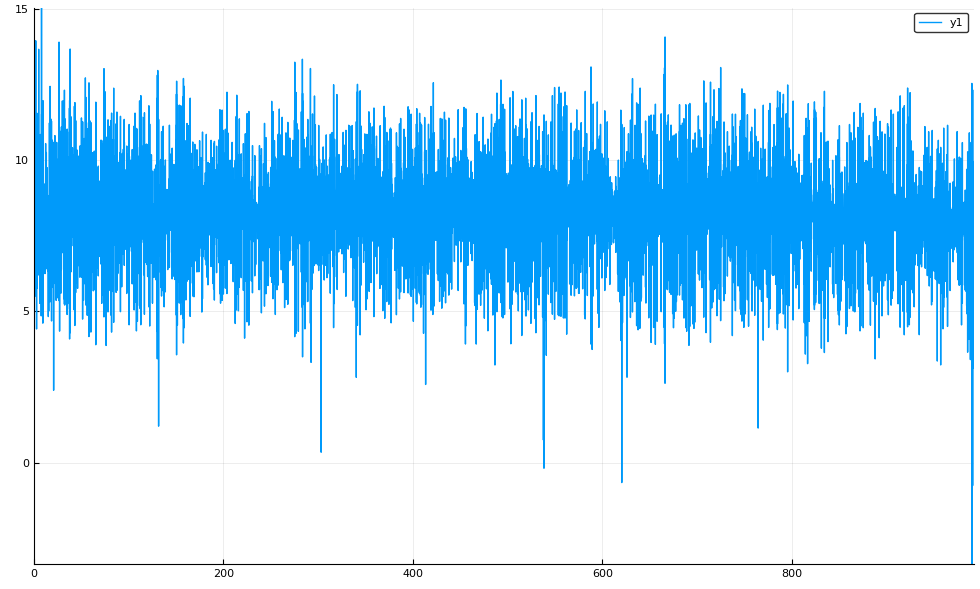
\includegraphics[width=\linewidth,height=\textheight,keepaspectratio]{images/accel_z}
\end{figure}
\end{frame}

\begin{frame} {Low Pass Filter}
\begin{figure}
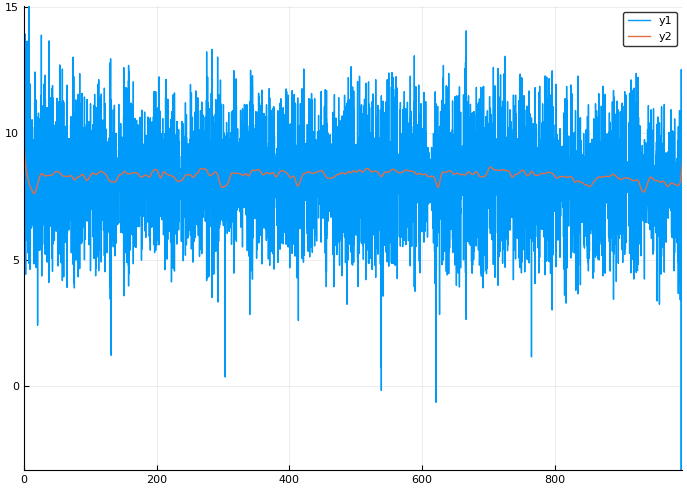
\includegraphics[width=\linewidth,height=\textheight,keepaspectratio]{images/accel_z_low}
\end{figure}
\end{frame}

\begin{frame} {Velocity Plot}
\begin{figure}
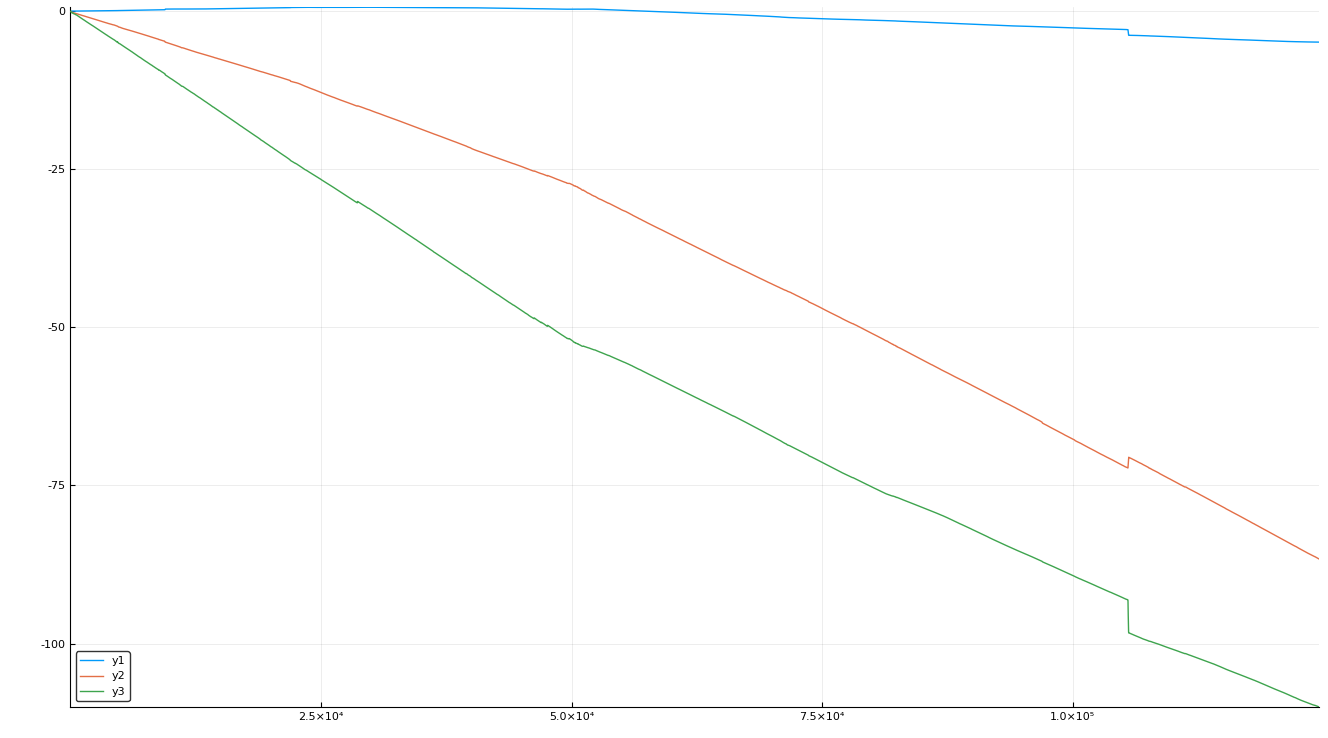
\includegraphics[width=\linewidth,height=\textheight,keepaspectratio]{images/velocity}
\end{figure}
\end{frame}

\begin{frame} {Position Plot}
\begin{figure}
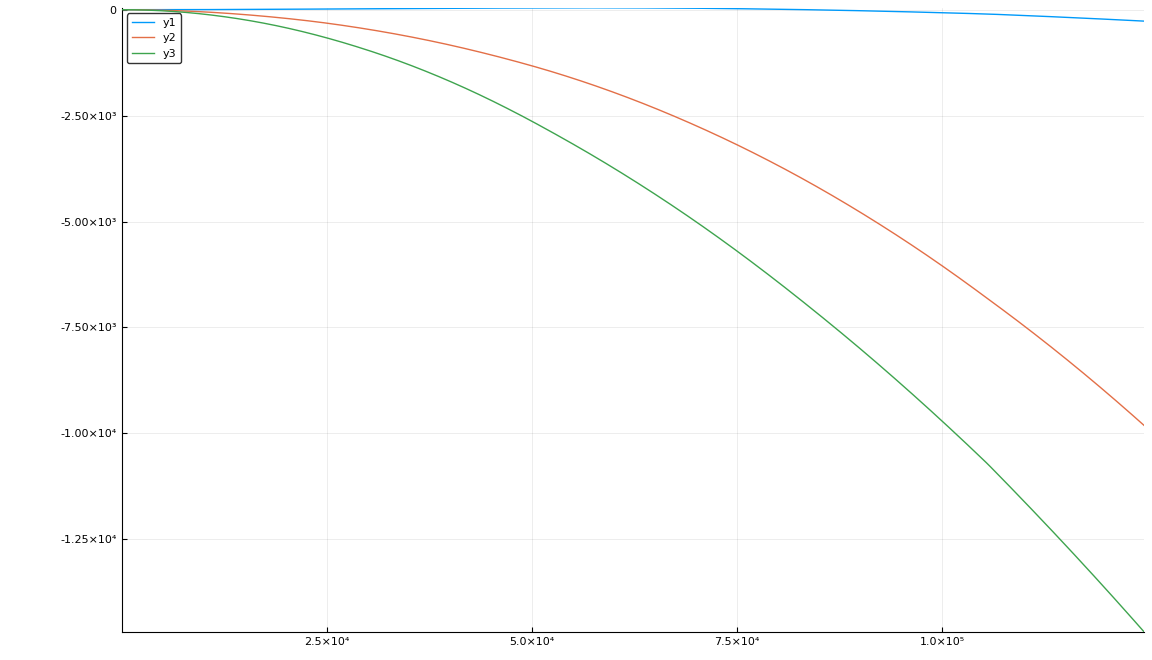
\includegraphics[width=\linewidth,height=\textheight,keepaspectratio]{images/position}
\end{figure}
\end{frame}

\begin{frame} {$SE(3)$}
If we can manage to process the accelerometer data to a high degree of accuracy, we will then try to map the position data and rotation data into $SE(3)$. From there we then plan on building a classification system that will classify such data and determine if the person is walking, mapping, or sitting as well as doing some other subtask. 
\end{frame}

\begin{frame}
\frametitle{References}
\bibliographystyle{plain}
\bibliography{references}
\end{frame}

\end{document}
